\begin{figure}
\centering
\begin{subfigure}[t]{0.4\textwidth}
\centering
\begin{tikzpicture}[scale=0.75,transform shape]
\GraphInit[vstyle=Simple]
\SetGraphUnit{2.5}
\Vertex[a=18,d=2.5]{A}
\Vertex[a=90,d=2.5]{B}
\Vertex[a=162,d=2.5]{C}
\Vertex[a=234,d=2.5]{D}
\Vertex[a=306,d=2.5]{E}
\Edge[label=$4$](A)(B)
\Edge[label=$3$](A)(D)
\Edge[label=$2$](B)(E)
\Edge[label=$5$](C)(D)
\Edge[label=$1$](D)(E)
\Edge[label=$2$,style={pos=0.7}](A)(C)
\Edge[label=$3$,style={pos=0.4}](C)(E)
\Edge[local,label=$1$,color=blue](B)(C)
\end{tikzpicture}
\caption{}
\end{subfigure}
\;
\begin{subfigure}[t]{0.4\textwidth}
\centering
\begin{tikzpicture}[scale=0.75,transform shape]
\GraphInit[vstyle=Simple]
\SetGraphUnit{2.5}
\Vertex[a=18,d=2.5]{A}
\Vertex[a=90,d=2.5]{B}
\Vertex[a=162,d=2.5]{C}
\Vertex[a=234,d=2.5]{D}
\Vertex[a=306,d=2.5]{E}
\Edge[label=$4$](A)(B)
\Edge[label=$3$](A)(D)
\Edge[label=$2$](B)(E)
\Edge[label=$5$](C)(D)
\Edge[label=$2$,style={pos=0.7}](A)(C)
\Edge[label=$3$,style={pos=0.4}](C)(E)
\Edge[local,label=$1$,color=blue](B)(C)
\Edge[local,label=$1$,color=blue](D)(E)
\end{tikzpicture}
\caption{}
\end{subfigure}

\vspace{10pt}
\begin{subfigure}[t]{0.4\textwidth}
\centering
\begin{tikzpicture}[scale=0.75,transform shape]
\GraphInit[vstyle=Simple]
\SetGraphUnit{2.5}
\Vertex[a=18,d=2.5]{A}
\Vertex[a=90,d=2.5]{B}
\Vertex[a=162,d=2.5]{C}
\Vertex[a=234,d=2.5]{D}
\Vertex[a=306,d=2.5]{E}
\Edge[label=$4$](A)(B)
\Edge[label=$3$](A)(D)
\Edge[label=$2$](B)(E)
\Edge[label=$5$](C)(D)
\Edge[label=$3$,style={pos=0.4}](C)(E)
\Edge[local,label=$1$,color=blue](B)(C)
\Edge[local,label=$1$,color=blue](D)(E)
\Edge[local,label=$2$,color=blue,style={pos=0.7}](A)(C)
\end{tikzpicture}
\caption{}
\end{subfigure}
\;
\begin{subfigure}[t]{0.4\textwidth}
\centering
\begin{tikzpicture}[scale=0.75,transform shape]
\GraphInit[vstyle=Simple]
\SetGraphUnit{2.5}
\Vertex[a=18,d=2.5]{A}
\Vertex[a=90,d=2.5]{B}
\Vertex[a=162,d=2.5]{C}
\Vertex[a=234,d=2.5]{D}
\Vertex[a=306,d=2.5]{E}
\Edge[label=$4$](A)(B)
\Edge[label=$3$](A)(D)
\Edge[label=$5$](C)(D)
\Edge[label=$3$,style={pos=0.4}](C)(E)
\Edge[local,label=$1$,color=blue](B)(C)
\Edge[local,label=$1$,color=blue](D)(E)
\Edge[local,label=$2$,color=blue,style={pos=0.7}](A)(C)
\Edge[local,label=$2$,color=blue](B)(E)
\end{tikzpicture}
\caption{}
\end{subfigure}
\caption{%
The execution of Kruskal's algorithm on a weighted graph $G$. Blue edges are
part of the final MST of $G$ generated by the algorithm.
}
\label{fig:kruskal-example}
\end{figure}
